\documentclass[margin=2mm]{standalone}
\usepackage{tikz}
\usetikzlibrary{arrows.meta, positioning, calc, shapes.geometric}

\begin{document}

% --- Flowchart 1: Offline Model Pipeline ---
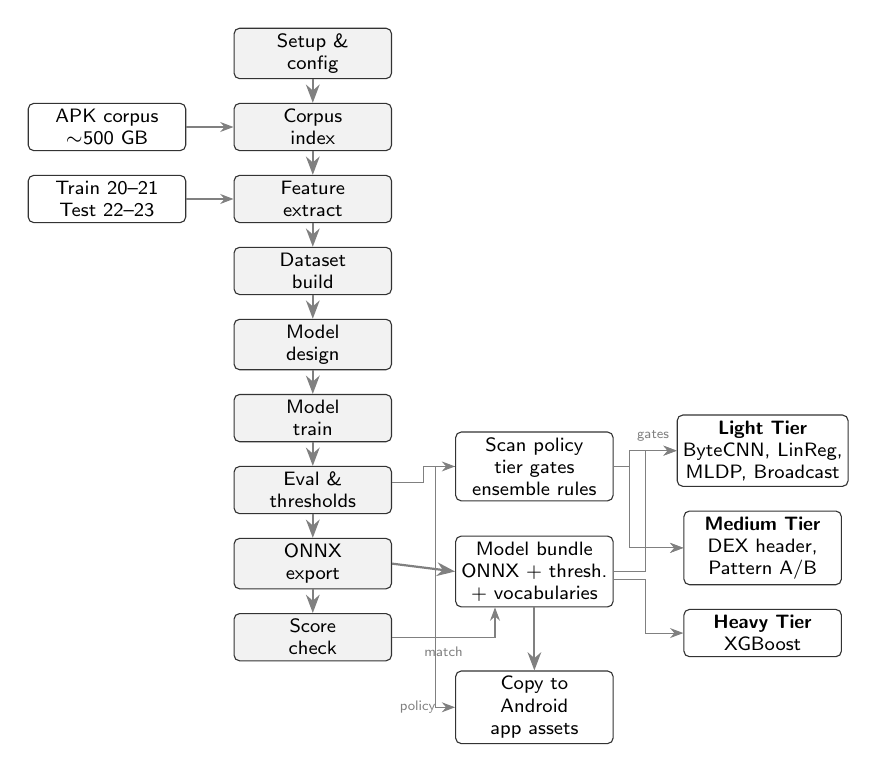
\begin{tikzpicture}[
  >=Stealth,
  box/.style={rectangle, draw=black!80, rounded corners=2pt, fill=gray!10, align=center, font=\sffamily\fontsize{7}{8}\selectfont, minimum width=2.0cm, minimum height=0.6cm, inner sep=2pt},
  sidebox/.style={rectangle, draw=black!80, rounded corners=2pt, fill=white, align=center, font=\sffamily\fontsize{7}{8}\selectfont, minimum width=2.0cm, minimum height=0.6cm, inner sep=2pt},
  tierbox/.style={rectangle, draw=black!80, rounded corners=2pt, fill=white, align=center, font=\sffamily\fontsize{7}{8}\selectfont, minimum width=2.0cm, minimum height=0.6cm, inner sep=2pt}
]

% Central column
\node[box] (c1) {Setup \&\\config};
\node[box, below=0.3cm of c1] (c2) {Corpus\\index};
\node[box, below=0.3cm of c2] (c3) {Feature\\extract};
\node[box, below=0.3cm of c3] (c4) {Dataset\\build};
\node[box, below=0.3cm of c4] (c5) {Model\\design};
\node[box, below=0.3cm of c5] (c6) {Model\\train};
\node[box, below=0.3cm of c6] (c7) {Eval \&\\thresholds};
\node[box, below=0.3cm of c7] (c8) {ONNX\\export};
\node[box, below=0.3cm of c8] (c9) {Score\\check};

\foreach \i/\j in {1/2, 2/3, 3/4, 4/5, 5/6, 6/7, 7/8, 8/9} {
  \draw[->, thick, gray] (c\i) -- (c\j);
}

% Left inputs
\node[sidebox, left=0.6cm of c2] (l1) {APK corpus\\$\sim$500 GB};
\draw[->, gray] (l1) -- (c2);

\node[sidebox, left=0.6cm of c3] (l2) {Train 20--21\\Test 22--23};
\draw[->, gray] (l2) -- (c3);

% Right side elements
\node[sidebox, right=0.8cm of c7, yshift=0.3cm] (r_pol) {Scan policy\\tier gates\\ensemble rules};
\node[sidebox, right=0.8cm of c8, yshift=-0.1cm] (r_bun) {Model bundle\\ONNX + thresh.\\+ vocabularies};
\node[sidebox, below=0.8cm of r_bun] (r_app) {Copy to\\Android\\app assets};

% Tiers: further right
\node[tierbox, right=0.8cm of r_pol, yshift=0.2cm] (t_light) {\textbf{Light Tier}\\ByteCNN, LinReg,\\MLDP, Broadcast};
\node[tierbox, below=0.3cm of t_light] (t_med) {\textbf{Medium Tier}\\DEX header,\\Pattern A/B};
\node[tierbox, below=0.3cm of t_med] (t_heavy) {\textbf{Heavy Tier}\\XGBoost};

% Connect right elements
\draw[->, gray] (c7.east) ++(0,0.1) -- ++(0.4,0) |- (r_pol.west);
\draw[->, gray, thick] (c8.east) -- (r_bun.west);
\draw[->, gray] (c9.east) -| node[pos=0.25, below, font=\sffamily\fontsize{5}{6}\selectfont] {match} ([xshift=-0.5cm]r_bun.south);

\draw[->, gray, thick] (r_bun.south) -- (r_app.north);
\draw[->, gray] (r_pol.west) -- ++(-0.25,0) |- node[pos=0.75, left, font=\sffamily\fontsize{5}{6}\selectfont] {policy} (r_app.west);

% Connect to Tiers
\draw[->, gray] (r_pol.east) -- ++(0.2,0) |- node[pos=0.75, above, font=\sffamily\fontsize{5}{6}\selectfont] {gates} (t_light.west);
\draw[->, gray] (r_pol.east) -- ++(0.2,0) |- (t_med.west);

\draw[->, gray] (r_bun.east) -- ++(0.4,0) |- (t_light.west);
\draw[->, gray] (r_bun.east) -- ++(0.4,0) |- (t_med.west);
\draw[->, gray] (r_bun.east) ++(0,-0.1) -- ++(0.4,0) |- (t_heavy.west);

\end{tikzpicture}


% --- Flowchart 2: On-Device Application Flow ---
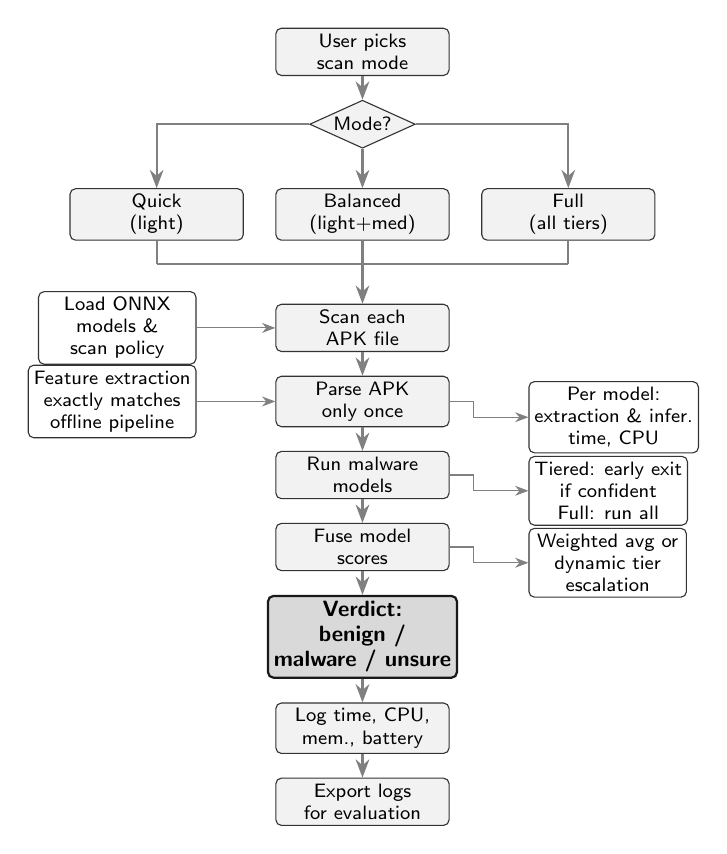
\begin{tikzpicture}[
  >=Stealth,
  box/.style={rectangle, draw=black!80, rounded corners=2pt, fill=gray!10, align=center, font=\sffamily\fontsize{7}{8}\selectfont, minimum width=2.2cm, minimum height=0.6cm, inner sep=2pt},
  dec/.style={diamond, aspect=2.2, draw=black!80, fill=gray!10, align=center, font=\sffamily\fontsize{7}{8}\selectfont, inner sep=1pt},
  sidebox/.style={rectangle, draw=black!80, rounded corners=2pt, fill=white, align=center, font=\sffamily\fontsize{7}{8}\selectfont, minimum width=2.0cm, minimum height=0.6cm, inner sep=2pt},
  verdict/.style={rectangle, draw=black!90, thick, rounded corners=2pt, fill=gray!30, align=center, font=\sffamily\fontsize{8}{9}\selectfont\bfseries, minimum width=2.4cm, minimum height=0.8cm, inner sep=2pt}
]

% Top section
\node[box] (s1) {User picks\\scan mode};
\node[dec, below=0.3cm of s1] (smode) {Mode?};
\draw[->, gray, thick] (s1) -- (smode);

% Mode branches
\node[box, below=0.5cm of smode] (b_bal) {Balanced\\(light+med)};
\node[box, left=0.4cm of b_bal] (b_qui) {Quick\\(light)};
\node[box, right=0.4cm of b_bal] (b_ful) {Full\\(all tiers)};

\draw[->, gray, thick] (smode.west) -| (b_qui.north);
\draw[->, gray, thick] (smode.south) -- (b_bal.north);
\draw[->, gray, thick] (smode.east) -| (b_ful.north);

% Main central flow
\node[box, below=0.8cm of b_bal] (scan) {Scan each\\APK file};

\draw[gray, thick] (b_qui.south) -- ++(0,-0.3) coordinate (m1);
\draw[gray, thick] (b_ful.south) -- ++(0,-0.3) coordinate (m2);
\draw[gray, thick] (m1) -- (m2);
\draw[->, gray, thick] (b_bal.south) -- (scan.north);

\node[box, below=0.3cm of scan] (parse) {Parse APK\\only once};
\node[box, below=0.3cm of parse] (run) {Run malware\\models};
\node[box, below=0.3cm of run] (fuse) {Fuse model\\scores};
\node[verdict, below=0.3cm of fuse] (verd) {Verdict:\\benign /\\malware / unsure};
\node[box, below=0.3cm of verd] (log) {Log time, CPU,\\mem., battery};
\node[box, below=0.3cm of log] (export) {Export logs\\for evaluation};

\foreach \i/\j in {scan/parse, parse/run, run/fuse, fuse/verd, verd/log, log/export} {
    \draw[->, gray, thick] (\i) -- (\j);
}

% Left Inputs
\node[sidebox, left=1cm of scan] (l_onnx) {Load ONNX\\models \&\\scan policy};
\node[sidebox, left=1cm of parse] (l_feat) {Feature extraction\\exactly matches\\offline pipeline};

\draw[->, gray] (l_onnx.east) -- (scan.west);
\draw[->, gray] (l_feat.east) -- (parse.west);

% Right outputs/annotations
\node[sidebox, right=1cm of parse, yshift=-0.2cm] (r_prep) {Per model:\\extraction \& infer.\\time, CPU};
\node[sidebox, right=1cm of run, yshift=-0.2cm] (r_tier) {Tiered: early exit\\if confident\\Full: run all};
\node[sidebox, right=1cm of fuse, yshift=-0.2cm] (r_fuse) {Weighted avg or\\dynamic tier\\escalation};

\draw[->, gray] (parse.east) -- ++(0.3,0) |- (r_prep.west);
\draw[->, gray] (run.east) -- ++(0.3,0) |- (r_tier.west);
\draw[->, gray] (fuse.east) -- ++(0.3,0) |- (r_fuse.west);

\end{tikzpicture}

\end{document}
